% !TEX root = ../../../under-spec-z.tex

\subsection{Constructing Grothendieck topologies} % (fold)
\label{sub:constructing_grothendieck_topologies}

    \subsubsection{Exactness and pullbacks} % (fold)
    \label{ssub:exactness_and_pullbacks}

        \begin{definition}[Conservative functor]
            Let $F\colon\ccat\to\dcat$ be a functor.
            Then $F$ is \emph{conservative} if, for all morphisms $f$ in $\ccat$, whenever the morphism $F(f)$ in $\dcat$ is an isomorphism then so too is $f$.
        \end{definition}

        \begin{definition}[Exact functor]
            Let $F$ be a functor.
            We say that $F$ is \emph{left exact} if it commutes with finite limits.
            Dually, $F$ is \emph{right exact} if it commutes with finite colimits.
            If $F$ is both left and right exact, then we say that it is \emph{exact}.
        \end{definition}

        If $F\colon\ccat\to\dcat$ where $\ccat$ and $\dcat$ both have zero objects then, loosely speaking, $F$ being conservative is saying that\footnote{
            If we wanted to really abuse notation then we would write this as $F^{-1}(0)=\{0\}$.
        } $[F(c)=0\implies c=0]$, and $F$ being exact is saying that $F(0)=0$.

        \begin{lemma}\label{le:adjoint-and-commuting-with-limits}
            Let $(F\dashv G)$ be an adjunction of functors.
            Then $F$ commutes with colimits and $G$ commutes with limits.
            % Let $F$ be some functor that has a left adjoint (or, equivalently, \emph{is} a right adjoint).
            % Then $F$ commutes with limits.
            % Dually, let $G$ be some functor that has a right adjoint (or, equivalently, \emph{is} a left adjoint).
            % Then $G$ commutes with colimits.
        \end{lemma}

        \begin{proof}
            \cite[\S V.5, p.118]{Lane:1998fe}
        \end{proof}

        \begin{corollary}\label{co:adjoint-exactness}
            Left-adjoint functors are right exact; right-adjoint functors are left exact.
        \end{corollary}

        \begin{definition}[Pullbacks]\label{df:pullbacks}
            Let $\ccat$ be a category, $X,X',Y\in\ccat$ objects, and $f\colon X\to Y$, $g\colon X'\to Y$ morphisms:
            \begin{equation*}
                \begin{tikzcd}[row sep=.7em]
                    X \arrow[dr, "f"] &\\
                     & Y\\
                    X' \arrow[ur, swap, "g"] &
                \end{tikzcd}
            \end{equation*}
            Then the \emph{pullback} (or \emph{fibred product}) \emph{of $Y$ (along $f$ and $g$)} is the limit of this diagram (if it exists) and is written as $X\prescript{f}{}{\times}^g_Y X'$ (or just $X\times_Y X'$ when no confusion may arise).
            The commutative diagram
            \begin{equation*}
                \begin{tikzcd}[row sep=.7em]
                     & X \arrow[dr, "f"] &\\
                    X\times_Y X' \arrow[ur, "\pi_X"] \arrow[dr, swap, "\pi_{X'}"] & & Y\\
                     & X' \arrow[ur, swap, "g"] &
                \end{tikzcd}
            \end{equation*}
            is also called a \emph{cartesian square}.
        \end{definition}

        Since the pullback is a limit, if our category $\ccat$ has finite limits then it has pullbacks.
        In $\Set$, the pullback $X\times_A Y$ is given by `intersecting' the images of $X$ and $Y$ in $A$:
        \begin{equation*}
            X\times_A Y = \{(x,y)\in X\times Y\mid f(x)=g(y)\}.
        \end{equation*}
        Working in $\Op{T}$ for some topological space $T$ -- the category whose objects are open sets of $T$ and whose morphisms are the inclusion maps of the open sets -- pullbacks correspond to intersections (\cref{fg:opTandpullbacks}).
        So pullbacks generalise intersection, but also \emph{fibres}: let $Y,T$ be topological spaces, $p\in T$ some point with inclusion map $\iota\colon \{p\}\hookrightarrow T$, and $f\colon Y\to T$ continuous.
        Then the pullback is the \emph{fibre} (or \emph{preimage}) \emph{of $p$ under $f$}:
        \begin{equation*}
            Y\times_T \{p\}=\{y\in Y\mid f(y)=p\}.
        \end{equation*}
        (\cref{fg:pullback-as-fibre}).
        So when we have a continuous $\tau\colon S\to T$ we can think of $Y\times_T S$ as the \emph{fibre of the points of $\tau(S)\subset T$ under $f$}.

        \begin{figure}[h]
            \centering
            \begin{minipage}{0.4\textwidth}
                \centering
                \frame{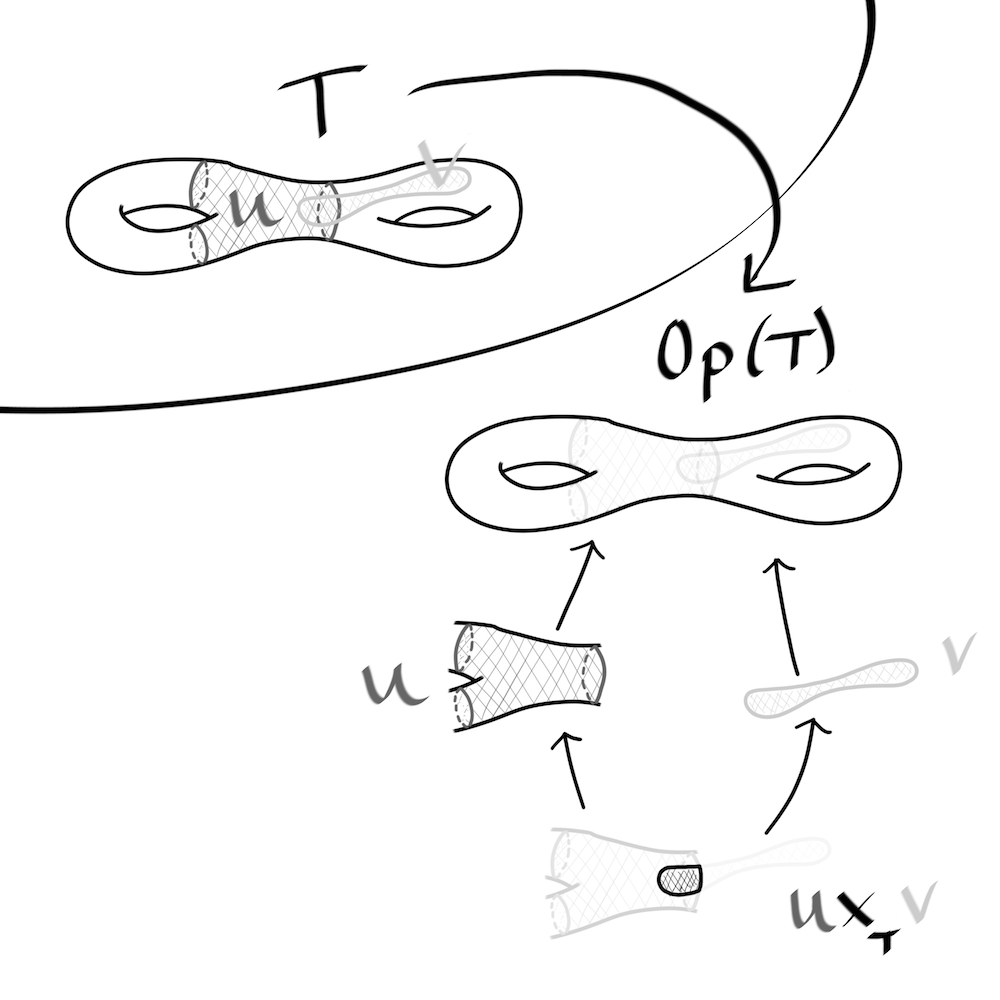
\includegraphics[width=\textwidth]{images/opTandpullbacks.png}}
                \caption{Pullbacks in $\Op{T}$}
                \label{fg:opTandpullbacks}
            \end{minipage}
            \hfill
            \begin{minipage}{0.59\textwidth}
                \centering
                \frame{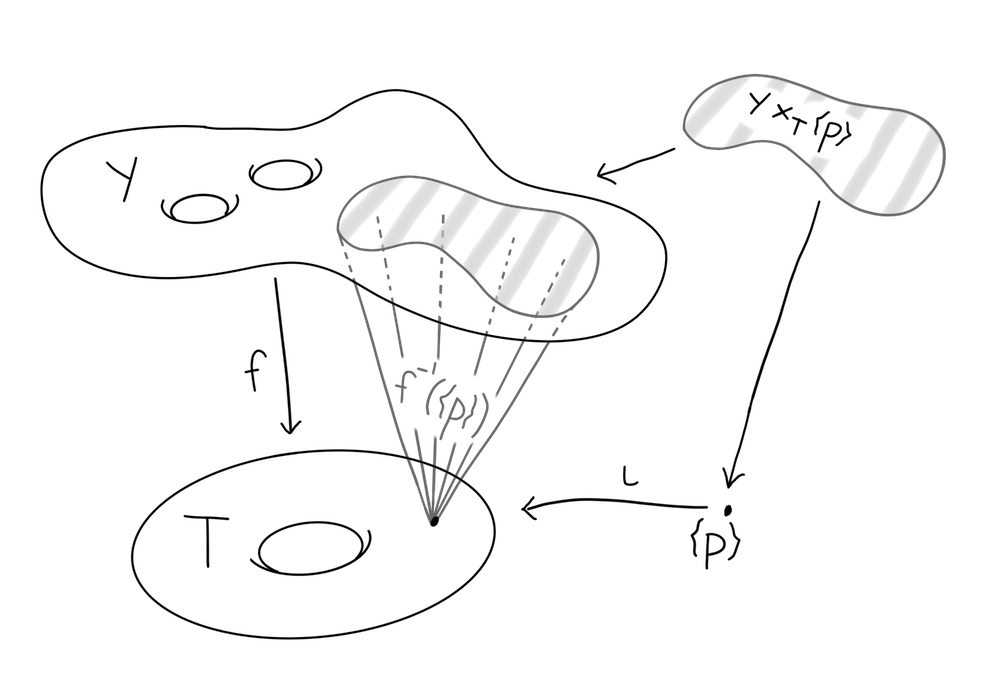
\includegraphics[width=\textwidth]{images/pullback-as-fibre.png}}
                \caption{Pullbacks as fibres}
                \label{fg:pullback-as-fibre}
            \end{minipage}
        \end{figure}

        % \begin{figure}[h]
        %     \centering
        %     \frame{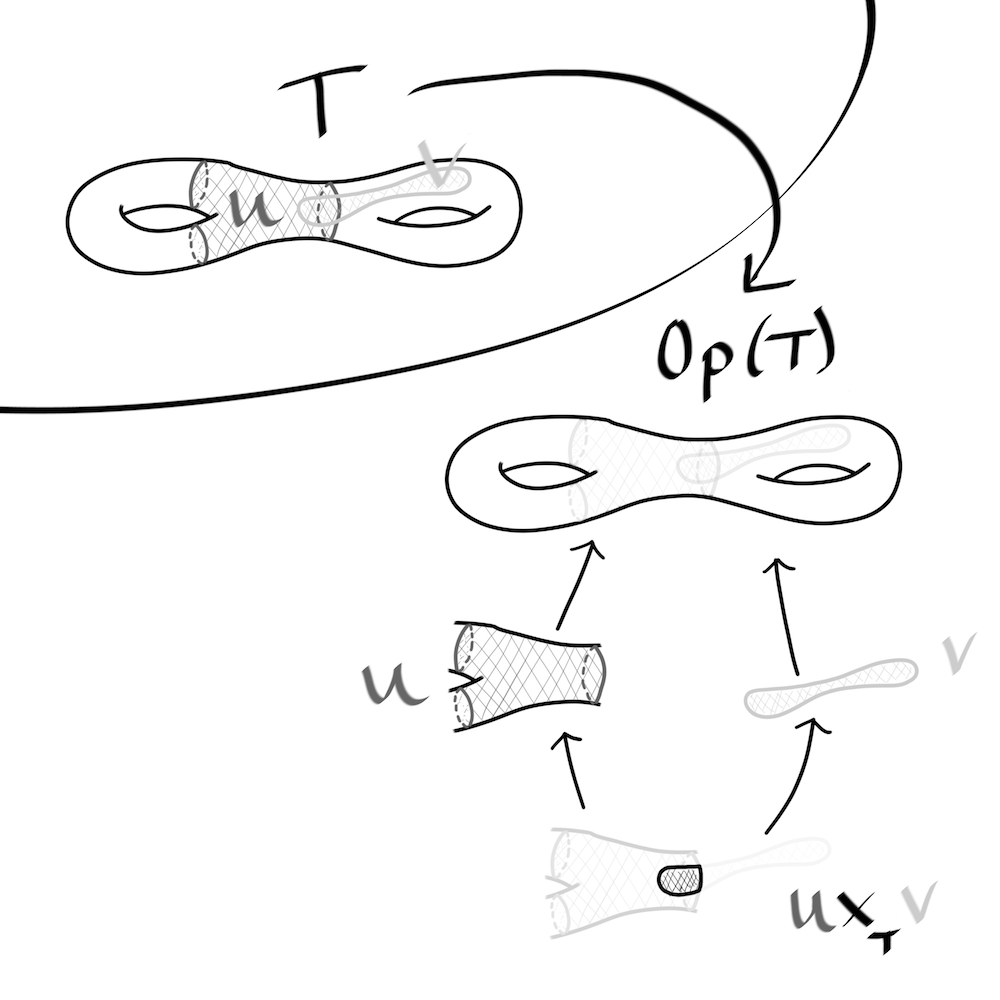
\includegraphics[width=.65\textwidth]{images/opTandpullbacks.png}}
        %     \caption{Pullbacks in $\Op{T}$}
        %     \label{fg:opTandpullbacks}
        % \end{figure}

    % subsubsection exactness_and_pullbacks (end)





    \subsubsection{Grothendieck pseudofunctor} % (fold)
    \label{ssub:a_useful_pseudofunctor}
    
        \begin{definition}[Grothendieck pseudofunctor\footnote{
            This is not standard terminology, but aims to hint at the links to \emph{Grothendieck fibrations} and the \emph{Grothendieck construction}.
            We should probably instead call $M$ a \emph{$\tcat$-indexed category with $\tcat$-indexed coproducts} (see \cite[Definitions~2.1,~3.1]{Ponto:2012wl}).
        } {(Hypothèse~2.1, \S2.1, p.8)}]\label{df:m-t-grothendieck-setup}
            Let $\tcat$ be a category that has finite limits and $M\colon\op{\tcat}\to\Cat$ a pseudofunctor\footnote{
                That is, a `not-quite-functor' $\tcat\to\Cat$ (the category of small categories), in the sense that it doesn't necessarily preserve composition of morphisms and the identity morphism \emph{exactly}, but only up to \emph{coherent isomorphism}.
                Roughly speaking, we require a natural isomorphism $F(g\circ f)\cong F(g)\circ F(f)$ such that we can `evaluate' $F(h)\circ F(g)\circ F(f)$ in an associative way.
                There is a similar condition concerning the identity morphism.
                For more details see \cite[Definition~7.5.1, \S7.5, p.296]{Borceux:1994ws}.
            }.
            Then $M$ is a \emph{Grothendieck pseudofunctor} if it satisfies the following conditions:
            \begin{enumerate}[(i)]
                \item for each $X$ in $\tcat$, the category $M(X)$ has all limits and colimits;
                \item for each $p\colon X'\to X$ in $\tcat$, the functor $M(p)=p^*\colon M(X)\to M(X')$ has a right adjoint $p_*\colon M(X')\to M(X)$ that is conservative;
                \item (\emph{the Beck-Chevalley condition}) for all pullbacks
                    \begin{equation*}
                        \begin{tikzcd}[row sep=.7em]
                             & Y \arrow[dr, "q"] &\\
                            X\times_Z Y \arrow[ur, "p'"] \arrow[dr, swap, "q'"] & & Z\\
                             & X \arrow[ur, swap, "p"] &
                        \end{tikzcd}
                    \end{equation*}
                    in $\tcat$, the natural transformation $p^*q_*\nt q'_*(p')^*$ (called the \emph{change of base}\footnote{
                        See \cref{nt:change-of-base} for information on this terminology.
                    }) is an isomorphism.
                    (\emph{See \cite[\S2,~\P3]{Toen:2005wxa} for how this transformation is constructed}).\qedhere
                    % (See the translation below and \cref{nt:change-of-base})\qedhere
            \end{enumerate}
        \end{definition}

        % \vspace{-2em}

        % \begin{translation}{2}{3}
        %     As a note on condition (iii), the natural transformation in question is constructed in the following way.
        %     We have the natural isomorphisms
        %     \begin{equation*}
        %         (q')^*p^* \cong (pq')^* = (qp')^* \cong (p')^*q^*
        %     \end{equation*}
        %     coming from $M$ being a pseudofunctor.
        %     This gives us, by composing on the right by $q_*$, a natural isomorphism $(q')^*p^*q_*\cong(p')^*q^*q_*$.
        %     By further composing this with the counit $q^*q_*\nt\id$ of the adjuction, we find a natural transformation
        %     \begin{equation*}
        %         (q')^*p^*q_*\nt(p')^*
        %     \end{equation*}
        %     which, by adjuction, gives us
        %     \begin{equation*}
        %         p^*q_*\nt q'_*(p')^*.
        %     \end{equation*}
        %      This is the change of base natural transformation.
        % \end{translation}

        The motivating example for such a pseudofunctor $M$ is when \emph{$\tcat$ is the category of affine schemes and \elide $M(X)$ is the category of quasi-coherent sheaves on $X\in\tcat$} (Remarque~2.2, \S2.1, p.9).

        \begin{figure}[h]
            \centering
            \frame{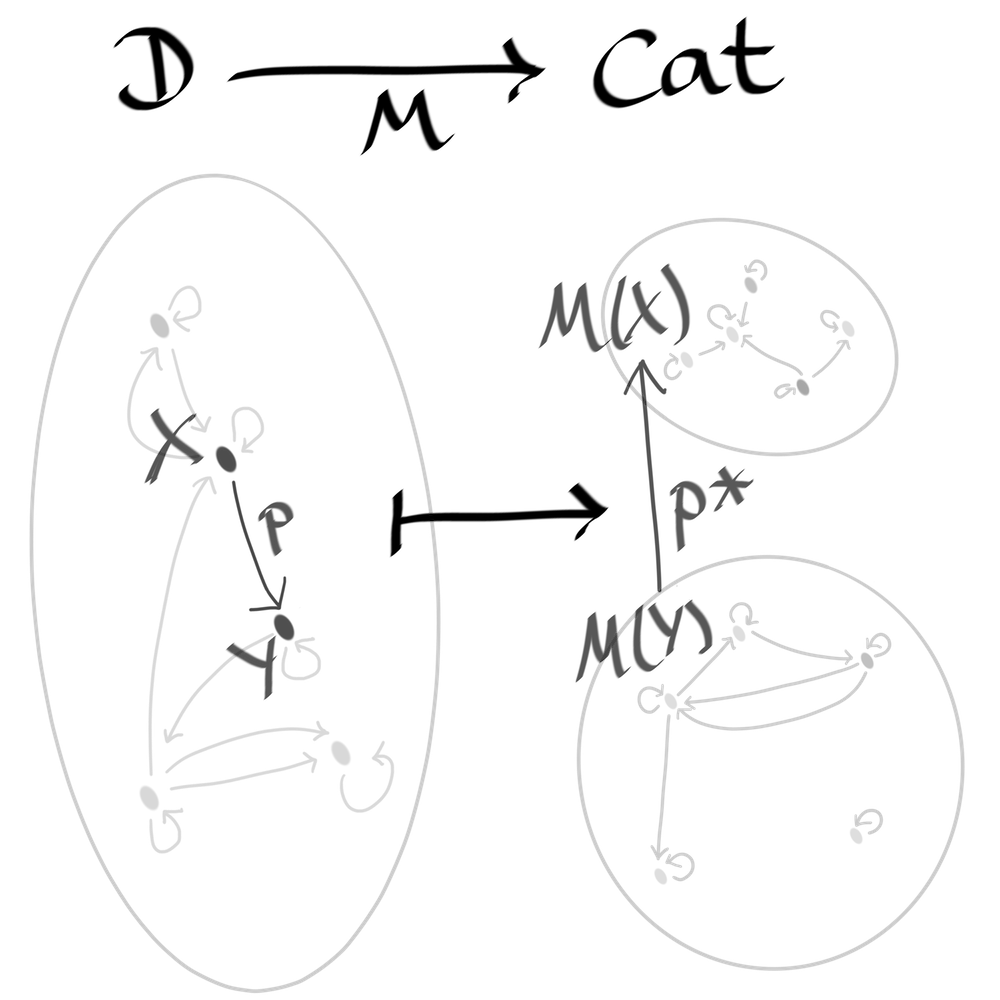
\includegraphics[width=.55\textwidth]{images/grothendieckpseudofunctor.png}}
            \caption{\cref{df:m-t-grothendieck-setup} – note that this is a picture of a contravariant $M\colon\dcat\to\Cat$ rather than a covariant $M\colon\op{\dcat}\to\Cat$.}
            \label{fg:grothendieckpseudofunctor}
        \end{figure}

        \begin{definition}[$M$-faithfully flat {(Définition~2.3, \S2.1, p.9)}]
            Let $\tcat$ and $M$ be as in \cref{df:m-t-grothendieck-setup}, and let $\famofmor$ be a family of morphisms in $\tcat$.
            Then $\famofmor$ is
            \begin{enumerate}[(i)]
                \item \emph{$M$-covering} if there exists a finite (non-empty) subset $J\subset I$ such that the family of functors
                \begin{equation*}
                    \{p_j^*\colon M(X)\to M(X_j)\}_{j\in J}
                \end{equation*}
                is conservative;
                \item \emph{$M$-flat} if all the functors $p_i^*\colon M(X)\to M(X_i)$ are left exact\footnote{
                    Note that, by \cref{df:m-t-grothendieck-setup}, a morphism $p\colon X'\to X$ is $M$-flat if and only if the functor $p^*$ is \emph{exact}.
                    This is because left adjoint functors are right exact (\cref{co:adjoint-exactness}) and we have assumed that $p^*$ \emph{has} a right adjoint (\cref{df:m-t-grothendieck-setup}).
                };
                \item \emph{$M$-faithfully flat} if it is both $M$-covering and $M$-flat.\qedhere
            \end{enumerate}
        \end{definition}

        The reason for the name `$M$-faithfully flat' comes from the fact that \emph{if $p$ is $M$-faithfully flat then $p^*$ is faithful}\footnote{
            We provide here a quick proof.
            Since $M(X)$ is bicomplete we have a \emph{zero object} and the notion of an \emph{equaliser} (dual to \cref{df:coequaliser}).
            By definition, two morphisms $f,g$ in $M(X)$ are equal if and only if their equaliser is zero.
            Now $p^*$ is exact, so it commutes with limits.
            Thus $\eq(p^*(f)\rightrightarrows p^*(g))\cong\eq(p^*(f\rightrightarrows g))$.
            Further, since $p^*$ is exact, $p^*(0)=0$.
            Also, since $p^*$ is conservative, it reflects limits, so $[p^*(c)=0\implies c=0]$.
            Thus $p^*(c)=0$ if and only if $c=0$.
            Putting these facts together we see that $f=g$ if and only if $p^*(f)=p^*(g)$.
            That is, $p^*$ is faithful.
        } (\S2.1 \P5).

    % subsubsection a_useful_pseudofunctor (end)





    \subsubsection{Grothendieck topologies} % (fold)
    \label{ssub:grothendieck_topologies}
    
        Classically, we use a topology on a commutative $k$-algebra (or commutative ring) to define the notion of a \emph{sheaf}.
        One of the pivotal moments for algebraic geometry (and mathematics as a whole) was Groethendieck's generalisation of this idea in 1958, rephrased in terms of category theory (which was itself only around 13 years old).
        The foundational definition was that of a \emph{site}, which is a category endowed with a \emph{Grothendieck topology}\footnote{
            We sometimes refer to this simply as a \emph{topology}, but only when it is obvious what we mean.
        } -- a structure that mirrored that of open sets of a topological space\footnote{
            Though there is some confusion with this nomenclature; \cite{Johnstone:2002wb} suggests the name \emph{Grothendieck coverage}, but we stick with `topology' for simplicity.
            See \cite{Skoda:2011wq}.
        }.
        There is also a \emph{Grothedieck pretopology}, which is slightly less strict, but can be used to construct a topology.
        We formalise all of this below.

        \begin{definition}[Grothendieck pretopology {(\cite{Schreiber:8YBVOVEM})}]\label{df:grothendieck-pretopology}
            Let $\ccat$ be a category with pullbacks.
            A \emph{Grothendieck pretopology on $\ccat$} is an assignment, to each object $X\in\ccat$, of a collection $C(X)$ of families of morphisms to $X$, called \emph{covering families}, satisfying the following conditions for all $X\in\ccat$:
            \begin{enumerate}[(i)]
                \item (\emph{isomorphisms cover}) for every isomorphism $Y\congto X$ in $\ccat$, the singleton family $\{Y\congto X\}$ is in $C(X)$;
                \item (\emph{stability}) the collection $C(X)$ is stable under pullback (or change of base): if $\{X_i\to X\}\in C(X)$ and $f\colon Y\to X$ is some arbitrary morphism in $\ccat$, then $\{f^* X_i\to Y\}_{i\in I}\in C(Y)$, where $f^*X_i=(Y\times_X X_i)$;
                \item (\emph{transitivity}) if $\{X_i\to X\}_{i\in I}\in C(X)$ and there is a covering family $\{X_{i,j}\to X_i\}_{j\in J_i}\in C(X_i)$ for each $i\in I$, then the family of composites $\{X_{i,j}\to X_i\to X\}_{i\in I,j\in J_i}$ is also in $C(X)$.\qedhere
            \end{enumerate}
        \end{definition}

        \begin{figure}[h]
            \centering
            \frame{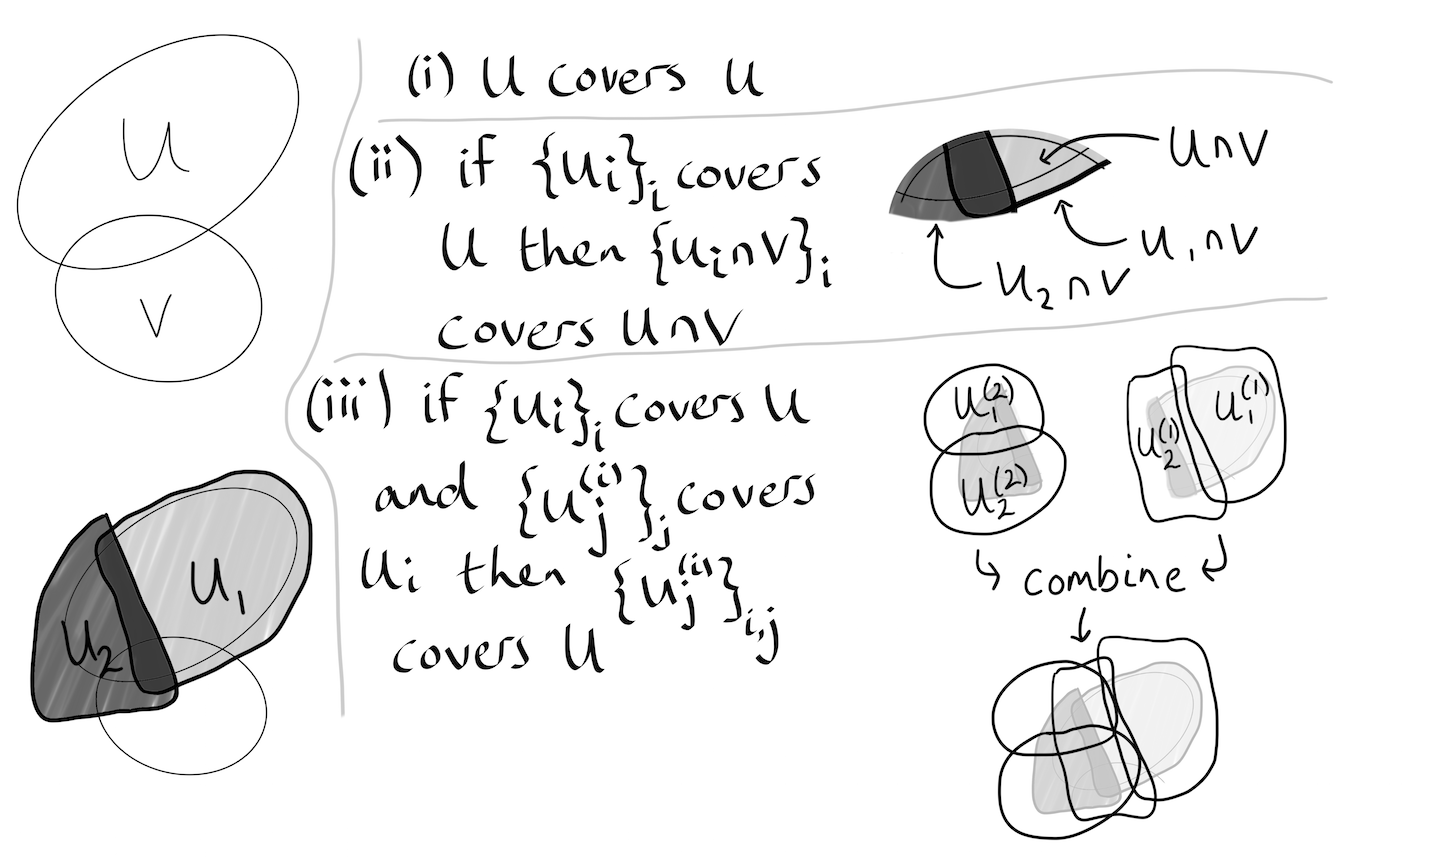
\includegraphics[width=.9\textwidth]{images/grothendieckpretopologyNEW.png}}
            \caption{\cref{df:grothendieck-pretopology} with $\ccat=\Op{T}$}
            \label{fg:grothendieckpretopology}
        \end{figure}

        The previously-introduced notion of `$M$-faithfully flat' now comes into use: such families can be used to construct a pretopology.

        \begin{lemma}[(Proposition~2.4, \S2.1, p.9)]\label{le:m-t-grothendieck-pretopology}
            Let $\tcat$ and $M$ be as in \cref{df:m-t-grothendieck-setup}.
            Then the $M$-faithfully flat families define\footnote{
                To each $X\in\tcat$ we assign the collection $C(X)$ of $M$-faithfully flat families $\{X_i\to X\}$.
            } a Grothendieck pretopology on $\tcat$.
        \end{lemma}

        \begin{proof}
            \mbox{}
            \begin{enumerate}[(i)]
                \item (\emph{Isomorphisms cover})
                    Let $p\colon Y\congto X$ be some isomorphism in $\dcat$.
                    We want $p^*\colon M(X)\to M(Y)$ to be conservative and left exact.
                    If we have $p^*\cong(p^{-1})_*$ then left exactness follows from being a right adjoint, and being conservative follows from \cref{df:m-t-grothendieck-setup}.

                    Since $M$ is a pseudofunctor, we have natural isomorphisms
                    \begin{align*}
                        (p^{-1})_*p_*\cong(pp^{-1})_*\cong&\id_{M(X)}\\
                        &\id_{M(Y)}\cong(p^{-1}p)_*\cong p_*(p^{-1})_*
                    \end{align*}
                    Thus $(p^{-1})_*\dashv p_*$ and so $(p^{-1})_*\cong p^*$ as required.
                \item (\emph{Stability})
                    Let $\{p_i\colon X_i\to X\}$ be $M$-faithfully flat and $f\colon Y\to X$.
                    Define $Y_i=Y\times_X X_i$ with morphisms
                    \begin{equation*}
                        \begin{tikzcd}[column sep=1em, row sep=.5em]
                            & Y \arrow[dr, "f"] &\\
                            Y_i \arrow[ur, "q_i"] \arrow[dr, swap, "f_i"] & & X\\
                            & X_i \arrow[ur, swap, "p_i"] &
                        \end{tikzcd}
                    \end{equation*}
                    We want to show that $\{q_i\colon Y_i\to Y\}$ is $M$-faithfully flat.

                    Firstly, to be $M$-covering we want
                    \begin{equation*}
                        \left(\prod_{j\in J} q_j^*\right)\colon M(Y)\to \prod_{j\in J} M(Y_j)
                    \end{equation*}
                    to be conservative for some finite $J\subset I$.
                    We claim that the same finite $J\subset I$ that makes $\{p_i\}$ $M$-covering works.
                    By \cref{df:m-t-grothendieck-setup}, $(f_i)_*$ is conservative, and so the above morphism is conservative if and only if
                    \begin{equation*}
                        \left(\prod_{j\in J} (f_j)_*q_j^*\right)\colon M(Y)\to \prod_{j\in J} M(X_j)
                    \end{equation*}
                    is conservative.
                    Now, $p_i^*f_*\cong(f_i)_*q_i^*$, so the above morphism is conservative if and only if
                    \begin{equation*}
                        \left(\prod_{j\in J} p_i^* f_*\right)\colon M(Y)\to \prod_{j\in J} M(X_j)
                    \end{equation*}
                    is conservative.
                    But both $f_*$ and $\{p_j^*\}_{j\in J}$ are conservative, so we are done.

                    Secondly, to be $M$-flat we want $q_i^*$ to be left exact for all $i\in I$.
                    This follows straight from $p_i^*f_*\cong(f_i)_*q_i^*$, since both $f_*$ and $(f_i)_*$ are right adjoints, thus left exact, and $p_i^*$ is left exact by hypothesis.
                \item (\emph{Transitivity})
                    Let $\{p_i\colon X_i\to X\}_{i\in I}$ be $M$-faithfully flat.
                    Suppose we also have $M$-faithfully flat $\{q^{(i)}_j\colon Y^{(i)}_j\to X_i\}_{j\in J}$ for all $i\in I$.
                    The fact that
                    \begin{equation*}
                        \{p_iq^{(i)}_j\colon Y^{(i)}_j\to X\}_{(i,j)\in I\times J}
                    \end{equation*}
                    is $M$-covering follows from the fact that the product of two finite sets is finite; that it is $M$-flat follows from the natural isomorphisms $(p_i q^{(i)}_j)^*\cong (q^{(i)}_j)^* p_i^*$ and the fact that the composition of two left-exact functors is again left exact.\qedhere
            \end{enumerate}
        \end{proof}

        \begin{definition}[Sieves on an object]
            Let $X\in\ccat$ be an object in some category.
            A \emph{sieve on $X$} is a subset\footnote{
                Again, we are assuming local smallness here for simplicity.
            } $S\subset \ccat/X$ of the objects of the slice category that is \emph{saturated} (i.e. closed under precomposition).
            That is, if $(Y\to X)\in S$ and $Y'\to Y$ is some arbitrary morphism in $\ccat$, then the composition $Y'\to Y\to X$ is also in $S$.
        \end{definition}

        If we have any collection $C$ of morphisms to some fixed object $X\in\ccat$ then we can \emph{saturate} the collection to obtain a sieve on $X$ -- we can extend the collection to include all precompositions by arbitrary morphisms to any object that is the source of a morphism in $C$.

        \begin{definition}[Pullback sieve]\label{df:pullback-sieve}
            Let $\ccat$ be some category, $S$ a sieve on $X\in\ccat$, and $f\colon Y\to X$ some morphism in $\ccat$.
            Then the \emph{pullback of $S$ along $f$}, written $f^* S$, is the sieve on $Y$ defined by\footnote{
                Roughly speaking, take all morphisms to $X$ that factor through $Y$ along $f$ and `divide them by $f$'.
            }
            \begin{equation*}
                f^* S = \{g\in\Hom(Y', Y) \mid Y\in\ccat,fg\in S\}.\qedhere
            \end{equation*}
        \end{definition}

        As to why this construction is called a pullback, we recall \cref{df:pullbacks} and claim that $f^* S$ is the image\footnote{
            Which we can avoid defining category-theoretically here since we have a natural underlying set structure.
        } of the projection
        \begin{equation*}
            S\times_{\Hom(\blank, X)}\Hom(\blank, Y) \to \Hom(\blank, Y)
            % \begin{array}{c}
                % S\times_{\Hom(\blank, X)}\Hom(\blank, Y)\\
            %     \Big\downarrow\\
            %     \Hom(\blank, Y)
            % \end{array}
        \end{equation*}
        where we take the pullback in $\Set$, and our morphisms are the inclusion $S\hookrightarrow\Hom(\blank, X)$ and post composition $(f\circ\blank)\colon\Hom(\blank, Y)\to\Hom(\blank, X)$.
        It follows from \cref{df:pullbacks} that, in $\Set$, the pullback is given by
        \begin{equation*}
            X\prescript{\varphi}{}{\times}^\psi_Z Y = \{(x,y)\in X\times Y \mid \varphi(x)=\psi(y)\}.
        \end{equation*}
        So here,
        \begin{equation*}
            S\times_{\Hom(\blank, X)}\Hom(\blank, Y) = \{(g,h)\in S\times\Hom(\blank, Y) \mid g=f\circ h\}
        \end{equation*}
        and projecting this to $\Hom(\blank, Y)$ gives the set of all morphisms $h$ such that $f\circ h=g$ for some $g\in S$.
        This is exactly what \cref{df:pullback-sieve} says.

        \begin{definition}[Grothendieck topology\footnote{
            As in \cite{Schreiber:2009wl}.
        }]\label{df:grothendieck-topology}
            Let $\ccat$ be some category.
            A \emph{Grothendieck topology on $\ccat$} is an assignment, to each object $X\in\ccat$, of a collection $J(X)$ of sieves on $X$, called \emph{covering sieves}, such that the following conditions are satisfied for all $X\in\ccat$:
            \begin{enumerate}[(i)]
                \item (\emph{base change}) if $S\in J(X)$ and $f\colon Y\to X$ is some arbitrary morphism in $\ccat$, then the pullback sieve satisfies $f^* S\in J(Y)$;
                \item (\emph{maximal sieve}) $\Hom(\blank,X)\in J(X)$;
                \item (\emph{intersections})\footnote{
                    This condition is actually redundant; see the comments after \cite[Definition~1,~\S III.2]{MacLane:1992uz}.
                } $S,T\in J(X)$ if and only if $S\cap T\in J(C)$;
                \item (\emph{transitivity}) if $S\in J(X)$ is such that $T_S\in J(X)$, where
                    \begin{equation*}
                        T_S=\bigcup_{Y\in\ccat}\{f\colon Y\to X \mid f^* S\text{ is covering on }Y\},
                    \end{equation*}
                    then $S\in J(X)$.\qedhere
            \end{enumerate}
        \end{definition}

        \begin{definition}[Site]\label{df:site}
            Let $\ccat$ be a category and $J$ a Grothendieck topology on $\ccat$.
            Then the pair $(\ccat,J)$ is called a \emph{site}.
        \end{definition}

        Recall: a pretopology on a category $\ccat$ consists of, for each $X\in\ccat$, a collection $C(X)$ of covering families $\{X_j\to X\}$.
        We can use these to pick certain sieves on $X$ that we wish to be in $J(X)$, and then see that this choice satisfies the conditions of \cref{df:grothendieck-topology}.
        The actual method is quite simple: given some sieve $S=\{S_i\to X\}$ on $X$, we say that $S\in J(X)$ if and only if it contains some covering family $\{X_j\to X\}\in C(X)$.
        More details on this construction can be found in \cite[\S III.2]{MacLane:1992uz}.

        % \begin{note}[Summary]\label{nt:make-topologies-with-m}
        %     \emph{The overall result of this section is as follows:} we can construct a Grothendieck topology on some category $\tcat$ (that has finite limits) by constructing some Grothendieck pseudofunctor $M$ and considering $M$-faithfully flat families.
        % \end{note}

        \begin{note}\label{nt:no-theorem-2.5}
            There is an important result (\cite[Théorème~2.5, \S2.1, p.11]{Toen:2005wxa}) that we don't cover here because it deals with the notion of \emph{stacks}.
            % Roughly speaking, a stack is like a sheaf, but whereas a sheaf is obtained by gluing together sets, a stack is obtained by gluing together categories.
            % Since categories have a much richer structure than sets (most notably, they have morphisms) the gluing is slightly more complicated, and needs the idea of \emph{descent data}, which is the abstract analogue of gluing.
            We do not have the space in this paper to cover the background needed to talk about stacks; we refer the interested reader back to \cite{Toen:2005wxa}.
            From now on we will skip over stack-theoretic theorems without mentioning them.
        \end{note}

    % subsubsection grothendieck_topologies (end)

% subsection constructing_grothendieck_topologies (end)
